\documentclass[11pt]{article}
\usepackage[margin=0.7in]{geometry}
\usepackage{amsmath,amssymb}
\usepackage{enumitem}
\usepackage{tikz}
\usepackage{pgfplots}
\pgfplotsset{compat=1.18}
\usepackage{fancyhdr}
\usepackage{parskip}
\setlist[enumerate]{leftmargin=*, itemsep=6pt}
\pagestyle{fancy}
\fancyhf{}
\fancyfoot[L]{\small\textit{en}Vision\textsuperscript{\textregistered} Algebra 2}
\fancyfoot[C]{\small 2-2 Lesson Quiz, short form}
\fancyfoot[R]{\small\thepage}
\renewcommand{\headrulewidth}{0pt}
\newcommand{\choice}[1]{\tikz[baseline=-0.6ex]\node[draw, circle, inner sep=0.6pt, minimum size=3.3mm, font=\scriptsize\bfseries] {#1};\;}
\newcommand{\checkbox}{$\square$\;}
\newcommand{\ansbox}[1][2.2cm]{\tikz[baseline=-0.8ex]\node[draw, rounded corners=3pt, minimum width=#1, minimum height=6mm] {};}
\pgfplotsset{quizgrid/.style={
  axis lines=middle, grid=both, grid style={gray!45},
  ticklabel style={font=\scriptsize, fill=white, inner sep=1pt},
  xlabel={$x$}, ylabel={$y$}, axis line style={thick}, clip=true}}

\begin{document}

\noindent\textbf{Name}\; \rule{6cm}{0.4pt} \hfill Period \rule{1.2cm}{0.4pt} \quad Date \rule{2.2cm}{0.4pt}

\vspace{4pt}\noindent\rule{\textwidth}{0.6pt}

\vspace{2pt}\noindent{\Large\textbf{2-2 \; Lesson Quiz: Standard Form of a Quadratic Function}} \hfill {\small short form}

\vspace{4pt}\noindent\rule{\textwidth}{0.6pt}

\vspace{6pt}
\textbf{2.} The amount of profit Bill makes per toy when he increases or decreases the price of his handmade toys can be modeled by the function $f(x)=-x^2-2x+3$. What price change gives him the highest profit? What is his highest profit per toy?

\vspace{6pt}
\begin{minipage}[t]{0.5\textwidth}
Price change: \$\,\ansbox

\vspace{8pt}
Maximum profit per toy: \$\,\ansbox
\end{minipage}\hfill
\begin{minipage}[t]{0.46\textwidth}
Show your work:

\vspace{4pt}\rule{\linewidth}{0.4pt}

\vspace{14pt}\rule{\linewidth}{0.4pt}

\vspace{14pt}\rule{\linewidth}{0.4pt}
\end{minipage}

\vspace{10pt}\noindent\rule{\textwidth}{0.4pt}

\vspace{6pt}
\textbf{3.} A pebble is tossed into the air from the top of a cliff. The height, in feet, of the pebble over time is modeled by the equation $y=-16x^2+32x+80$. What is the maximum height, in feet, reached by the pebble?

\vspace{6pt}
\begin{minipage}[t]{0.5\textwidth}
Maximum height: \ansbox \ ft
\end{minipage}\hfill
\begin{minipage}[t]{0.46\textwidth}
Show your work:

\vspace{4pt}\rule{\linewidth}{0.4pt}

\vspace{14pt}\rule{\linewidth}{0.4pt}

\vspace{14pt}\rule{\linewidth}{0.4pt}
\end{minipage}

\vspace{10pt}\noindent\rule{\textwidth}{0.4pt}

\vspace{6pt}
\begin{minipage}[t]{0.48\textwidth}
\textbf{5.} An equation that represents the path of a diver jumping off a diving board is $y=-7x^2+5x+16$. Graph this function from the point where the diver jumped to the point where they reach the water.

\vspace{8pt}
Show your thinking:

\vspace{4pt}
Where the diver jumped: $(\;\rule{1cm}{0.4pt}\;,\;\rule{1cm}{0.4pt}\;)$

\vspace{8pt}
Vertex: $(\;\rule{1cm}{0.4pt}\;,\;\rule{1cm}{0.4pt}\;)$

\vspace{8pt}
Reaches the water: about $(\;\rule{1cm}{0.4pt}\;,\;\rule{1cm}{0.4pt}\;)$
\end{minipage}\hfill
\begin{minipage}[t]{0.48\textwidth}
\vspace{-4pt}
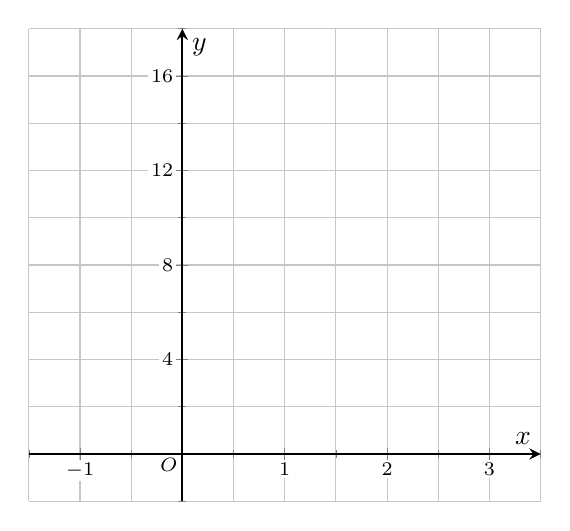
\begin{tikzpicture}
\begin{axis}[quizgrid, xmin=-1.5, xmax=3.5, ymin=-2, ymax=18,
  xtick={-1,1,2,3}, ytick={4,8,12,16}, minor xtick={-1.5,-1,...,3.5}, minor ytick={-2,0,...,18},
  x=1.3cm, y=0.3cm]
\node[font=\scriptsize, anchor=north east, inner sep=1.5pt] at (axis cs:0,0) {$O$};
\end{axis}
\end{tikzpicture}
\end{minipage}

\vfill
\noindent\textbf{Scoring:} Question 3 and Question 5 are 10 points each. Question 2 is a bonus of up to 5 points (2 for the price change, 3 for the profit). Total out of 20. (Question numbers are the Savvas quiz numbers; items 1 and 4 are on the full Savvas quiz only.)

\newpage
\noindent{\LARGE\textbf{2-2 Lesson Quiz, short form: answer key}}

\vspace{4pt}\noindent\rule{\textwidth}{0.6pt}

\begin{enumerate}
\item[\textbf{2.}] \textbf{Price change: \$$-1$. Maximum profit per toy: \$4.} $a=-1$, $b=-2$: $h=-\dfrac{b}{2a}=-\dfrac{(-2)}{2(-1)}=-1$, and $f(-1)=-1+2+3=4$. So lowering the price by \$1 gives the highest profit, \$4 per toy. Watch for $h=+1$ (the sign of $b$ dropped; the Common Error the TE flags for Try It 2), which gives $f(1)=0$. Savvas quiz item 2, DOK 2, skill F16 (Example 3). \textbf{Bonus 5:} 2 for $-1$ (accept ``decrease the price by \$1''), 3 for \$4.
\item[\textbf{3.}] \textbf{96 ft.} $h=-\dfrac{32}{2(-16)}=1$, and $y=-16(1)^2+32(1)+80=96$. Savvas quiz item 3, DOK 2, skill F16 (Example 3; Try It 3 is the same task). \textbf{10 points:} 4 for $h=1$ with the formula shown, 4 for substituting $x=1$ correctly, 2 for 96 ft.
\item[\textbf{5.}] \textbf{A downward parabola segment from $(0,16)$ to about $(1.91,0)$, vertex about $(0.36,\,16.89)$; closed endpoints, no arrows.} $h=-\dfrac{5}{2(-7)}=\dfrac{5}{14}\approx0.36$; $k=-7\!\left(\tfrac{5}{14}\right)^2+5\!\left(\tfrac{5}{14}\right)+16=16\tfrac{25}{28}\approx16.89$. The symmetric point of $(0,16)$ is $\left(\tfrac57,16\right)\approx(0.71,16)$. A table gives $y(1)=14$, $y(1.5)=7.75$, $y(2)=-2$, so the diver reaches the water between $x=1.5$ and $x=2$, near $x\approx1.91$. Savvas quiz item 5, DOK 2, skill F16 (Example 2 with Example 3's context). \textbf{10 points, all for the graph the TE asks for:} 2 for starting at $(0,16)$, 3 for a vertex near $(0.36,16.9)$, 3 for ending near $(1.9,0)$ (accept $1.8$--$2.0$), 2 for drawing only $0\le x\le 1.91$ with closed ends. The three ``show your thinking'' blanks are the same points written down; they earn these points when the graph is missing or unclear.
\end{enumerate}

\textbf{Items left off this form} (full Savvas quiz only; available for a retake or Form B): Savvas item 1, the minimum point of $f(x)=x^2-4x$ (answer D, $(2,-4)$; Example 1/2 vertex skill, DOK 2, F16); Savvas item 4, the parabola through $(-5,-10)$, $(-1,6)$ and $(2,-3)$ (answer A, $y=-x^2-2x+5$; Example 4, not taught in the fast packet, DOK 2, F50; students can still check each choice by substituting the three points).

\textbf{IXL replacement:} SmartScore 70 or above on L8C and S9G replaces this quiz with 20/20.

\end{document}
